\section{DShell - Análisis forense en redes}

%-----------------------    ---------------------------------

\begin{frame}
\frametitle{¿Qué es Dshell? ¿Y el análisis forense?}

\begin{itemize}
   \item Es un \emph{framework} de análisis forense en redes
   \item (Análisis forense: \emph {aplicación de técnicas científicas y analíticas especializadas a infraestructura tecnológica que permiten identificar, preservar, analizar y presentar datos que sean válidos dentro de un proceso legal.} \texttt{WikiPedia})
   \item Desarrollado por la U.S. Army
   \item Está en GitHub: \url{https://github.com/USArmyResearchLab/Dshell}
\end{itemize}

\end{frame}


%-----------------------    ---------------------------------

\begin{frame}
\frametitle{¿Para qué el análisis forense?}

\begin{itemize}
   \item La seguridad informática (especialmente en redes) es un tema que está siendo muy trabajado últimamente
   \item Wireshark es un analizador de tráfico visual, limitado para análisis forense
   \item Existen múltiples ataques
   \item Existen múltiples herramientas para atajar el problema
\end{itemize}

\end{frame}

%-----------------------    ---------------------------------

\begin{frame}
\frametitle{Dshell es una herramienta de la U.S. Army}

\begin{center}
  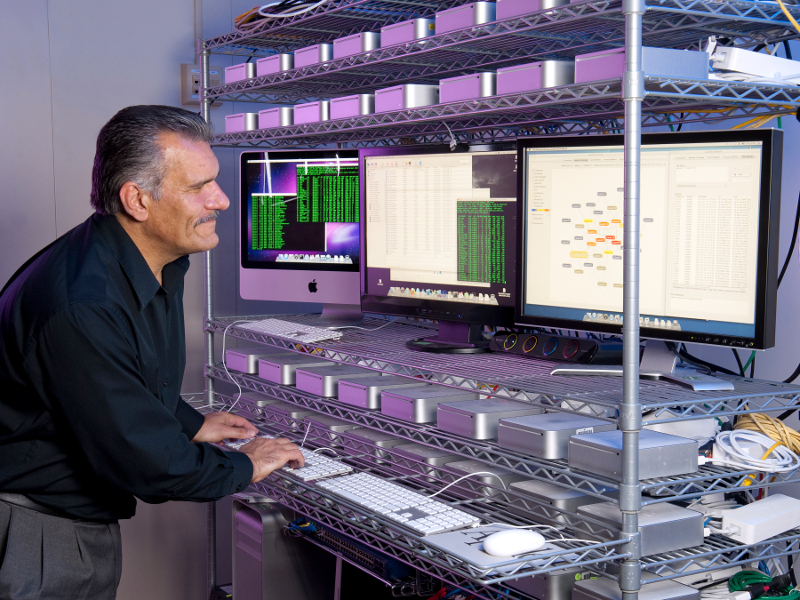
\includegraphics[width=10cm]{figs/dshell}
\end{center}


\begin{flushright}
{\tiny
Source: http://www.army.mil/media/379387/
}
\end{flushright}

\end{frame}



%-----------------------    ---------------------------------

\begin{frame}
\frametitle{No estás solo en Internet}

Posibles riesgos:

\begin{itemize}
  \item Pasivos
    \begin{itemize}
      \item wiretapping
      \item Port scanner
      \item Idle scan
    \end{itemize}
  \item Active
    \begin{itemize}
      \item Denial-of-service attack
      \item DNS spoofing
      \item Spoofing
      \item Man in the middle
      \item ARP poisoning
      \item Smurf attack
      \item Buffer overflow
      \item Heap overflow
      \item Format string attack
      \item SQL injection
      \item Cyber-attack
    \end{itemize}   
\end{itemize}

\end{frame}



